\documentclass[tikz,border=3pt,12pt]{standalone}
\usetikzlibrary{positioning,arrows.meta}
\begin{document}
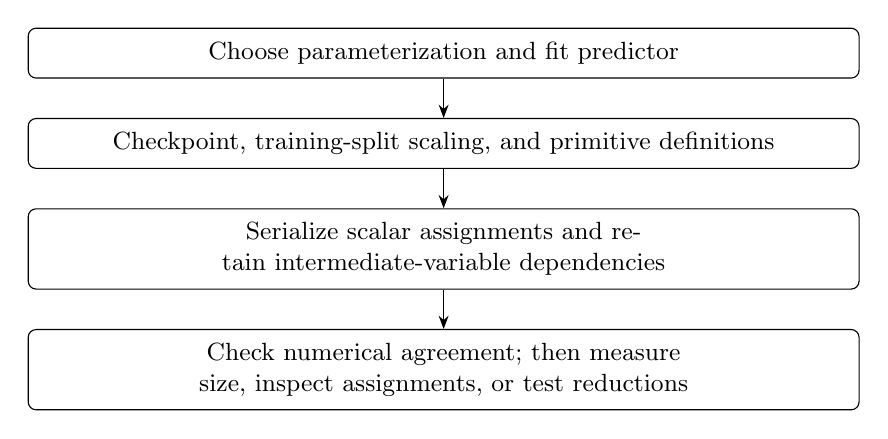
\begin{tikzpicture}[node distance=5mm, every node/.style={font=\small},
 stage/.style={draw,rounded corners=1mm,align=center,text width=10.2cm,inner sep=5pt}]
\node[stage] (a) {Choose parameterization and fit predictor};
\node[stage,below=of a] (b) {Checkpoint, training-split scaling, and primitive definitions};
\node[stage,below=of b] (c) {Serialize scalar assignments and retain intermediate-variable dependencies};
\node[stage,below=of c] (d) {Check numerical agreement; then measure size, inspect assignments, or test reductions};
\draw[-{Stealth}] (a)--(b);\draw[-{Stealth}] (b)--(c);\draw[-{Stealth}] (c)--(d);
\end{tikzpicture}
\end{document}
